\chapter{Test Results}
\label{ch5}

\section{GRU Test Dataset Performance Summary}
After determining the best model as applied to the validation dataset, the train and validation datasets are combined into an updated train dataset. The selected model is trained on the updated train dataset and then applied to the test dataset. Like in the grid search, 10 individual models are trained to evaluate convergence. Figure \ref{fig:GRU_train_test_loss_curves} illustrates the model training process by plotting the $log_{10}(C_{n}^{2})$ RMSE loss (evaluated between forecast and measured truth) as a function of training epoch. The blue curves represent each model's performance on the train dataset and the orange curves represent the performance on the test dataset. The solid and dashed black lines are the per-epoch average of the train and test dataset performances, respectively.
\begin{figure}[h!]
	\centering
	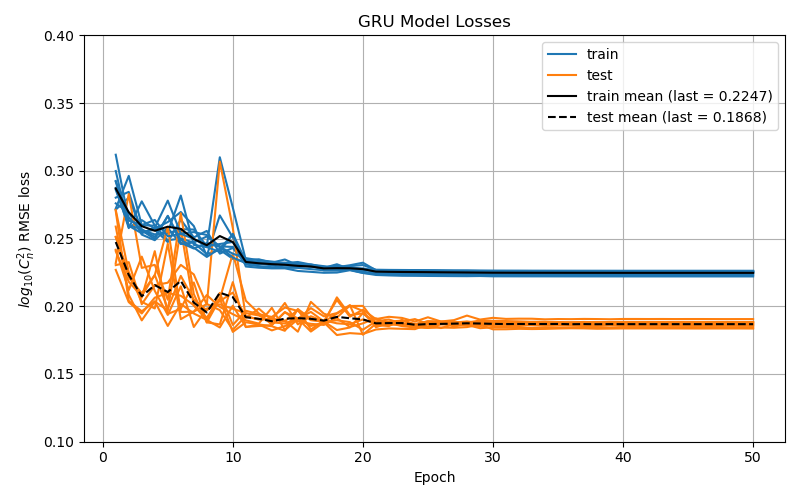
\includegraphics[width=0.75\textwidth]{GRU_loss_curves.png}
	\caption{GRU train and test loss curves of 10 models.}
	\label{fig:GRU_train_test_loss_curves}
\end{figure}
The loss curves in Figure \ref{fig:GRU_train_test_loss_curves} indicate that convergence rates of the models as applied to the train and test datasets are consistent with each other, an indication that the test dataset is a good representation of the train dataset. This is further illustrated by bumps in the loss scores in both train and validation loss curves like the single blue and orange spike at epoch 9. The per-epoch variability in the test dataset is higher than the train dataset since the test dataset is much smaller and thus more prone to changes in loss score with an update in model parameters. The 50th (last) epoch loss scores averaged over the 10 models are reported in the legend as 0.2247 and 0.1868 for the train and test dataset, respectively. The standard deviations of the 50th epoch loss scores for the train and test datasets are 0.0013 and 0.0020, respectively. As a point of comparison, the best MLP model was also trained then applied to the test dataset 10 times. The average 50th epoch loss scores are 0.2457 and 0.1938 with standard deviations of 0.0027990 and 0.0020191 for the train and test dataset, respectively. These results indicate that as applied to the test dataset, on average the chosen GRU model is better than the best MLP model by a large margin (\textcolor{blue}{add student's t-test p-value here to show significance?}), further validating the selection of the GRU model. The standard deviations of the test dataset loss scores are nearly identical, indicating the stability of the models are similar.

Another way to visualize model convergence is to apply the 10 individually-trained models to the test dataset parsed by day. The test dataset spans 08/03 and 08/05 - 08/10, so each model is evaluated on these seven days. The $log_{10}(C_{n}^{2})$ RMSE loss scores as a function of test day are illustrated in Figure \ref{fig:GRU_daily_performance}. Evaluated over the 10 models, in black is the mean, red the mean $\pm$ the standard deviation, and blue the minimum and maximum scores.
\begin{figure}[h!]
	\centering
	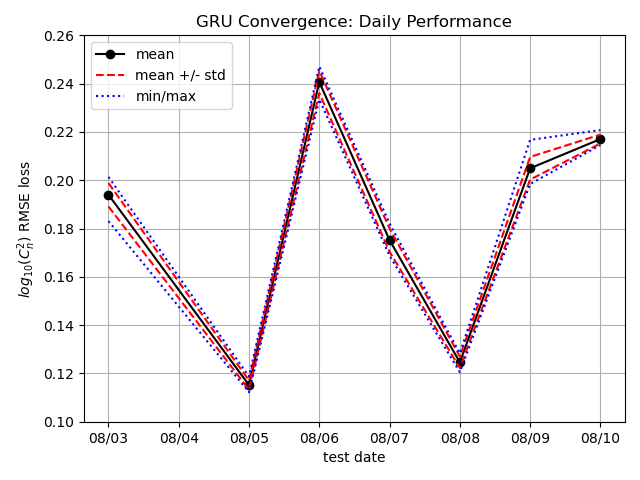
\includegraphics[width=0.65\textwidth]{GRU_daily_performance.png}
	\caption{GRU daily summary performance: mean, standard deviation, and min/max.}
	\label{fig:GRU_daily_performance}
\end{figure}
The day-to-day change in average error score, illustrated by the large jumps in error score like from 08/05 to 08/06, indicate that model performance varies by daily $C_{n}^{2}$ conditions. However, the tightness of the red and blue curves about the black markers indicate the models are converging to consistent solutions when evaluated on a daily basis. The largest difference between minimum and maximum loss scores is just less than 0.02 on 08/03 which is still a small variation in model performance for a given day. On 08/05 and 08/08 the red and blue lines are on top of the black markers indicating the model convergence is highly consistent when applied to these two days. These day-by-day results further confirm the test dataset loss curves in Figure \ref{fig:GRU_train_test_loss_curves} which indicate the models converge to a consistent solution when applied to the entire test dataset.

Another visualization of average model performance from the 10-model ensemble is presented in Figure \ref{fig:GRU_hourly_performance} which is the $log_{10}(C_{n}^{2})$ RMSE loss score of the test dataset parsed by the first timestep in each forecast. To make the plot in Figure \ref{fig:GRU_hourly_performance}, the 148 forecasts in the test dataset are sorted by the time of day of the first timestamp in each 4-hour forecast, the 30-minute forecast. The loss scores of each model applied to every test dataset forecast whose timestamp corresponds with a given time of day is plotted as the black markers. The average of the 10 loss scores are plotted as red markers for each test dataset forecast whose first timestamp is at the given time.
\begin{figure}[h!]
	\centering
	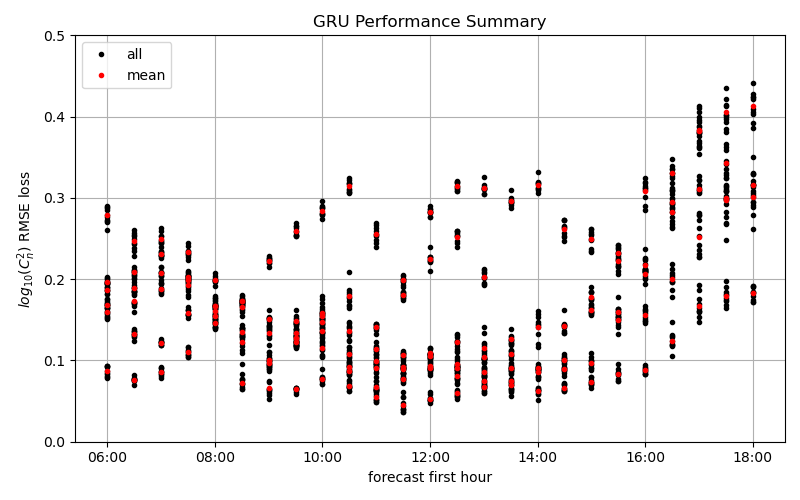
\includegraphics[width=0.65\textwidth]{GRU_hourly_performance.png}
	\caption{GRU hourly summary performance: individual and average.}
	\label{fig:GRU_hourly_performance}
\end{figure}
For example, evaluating the 06:00 (far left) time of day in Figure \ref{fig:GRU_hourly_performance} shows six red markers. This means that in the test dataset there are six forecasts whose first timestamp is at 06:00, and each red marker is the average loss (from the 10-model ensemble) for each of the six forecasts. The black dots at 06:00, of which there are 60 markers, are the model-by-model loss scores for each of the six forecasts. Still evaluating the 06:00 time of day, there is one red marker around 0.275 on the y-axis that is on top of a cluster of black points. This individual red marker is the average of the black markers which surround it. Thus, this cluster of black markers and their average, the red marker, is an evaluation of the ensemble model performance on one of the six forecasts whose first timestamp is at 06:00. Overall, Figure \ref{fig:GRU_hourly_performance} shows 148 red markers for the 148 forecasts in the test dataset, and 1480 black markers for the 10 models per 148 forecasts.

Figure \ref{fig:GRU_hourly_performance} is a summary of model performance as a function of time of day. The trends indicate that best model performance starts around 0.2 (on the y-axis) in the beginning of the day, drops down to around 0.1 in the middle of the day, then rises in the evening to around 0.3. The morning forecasts trend to be around the overall test dataset performance, about 0.18 to 0.20. On average, best performance is in the middle of the day between 11:00 and 15:00 since most of the black and red markers are clustered around 0.1 on the y-axis. In this window a few forecasts are consistently outliers (indicated by the red markers also being an outlier from the trend) in terms of error score. These individual forecasts are of interest for analysis. The high error scores at the end of the day, 16:00 to 18:00, is indicative that there are features of these late-day forecasts which are present in the measurements but are consistently not being captured by the ensemble of models. Generally, Figure \ref{fig:GRU_hourly_performance} indicates the model performs best in the middle of the day, slightly worse in the morning, and generally poorly in the late afternoon and evening.

\section{Daily $C_{n}^{2}$ Forecasts}
\label{sec:daily_cn2_forecasts}
After the ensemble study of the GRU models applied to the test dataset, a single GRU model is applied to the test dataset and carefully evaluated in this section. Figures \ref{fig:test_daily_results0} and \ref{fig:test_daily_results1} are daily-$C_{n}^{2}$ plots of the test forecasts and measured truth as a function of local time. Figures \ref{fig:test_daily_results0_a}, \ref{fig:test_daily_results0_b}, \ref{fig:test_daily_results0_c}, and \ref{fig:test_daily_results0_d} plot the forecasts on 08/03 and 08/05 - 08/07, respectively.  Figures \ref{fig:test_daily_results1_a}, \ref{fig:test_daily_results1_b}, and \ref{fig:test_daily_results1_c} plot the forecasts on 08/08 - 08/10, respectively. Each daily-$C_{n}^{2}$ plot contains multiple curves. The black curve represents the truth $C_{n}^{2}$ measured conditions. The other curves which transition in color from cyan to magenta represent the model forecasts throughout the day. The brightest cyan is the earliest forecast in the day, and the brightest magenta is the latest forecast in the day. The forecasts in between are appropriately colored to smoothly transition between the two end colors. The colorbar of each plot in Figures \ref{fig:test_daily_results0} and \ref{fig:test_daily_results1} illustrate the curve color scheme by labeling the forecast's first timestamp next to the color with which it's associated. Additionally, the $log_{10}(C_{n}^{2})$ RMSE loss score between each forecast and measured truth is also labeled in parenthesis next to the colorbars.
\begin{figure}[h!]
	\centering
	\subfloat[August 03\label{fig:test_daily_results0_a}]{
		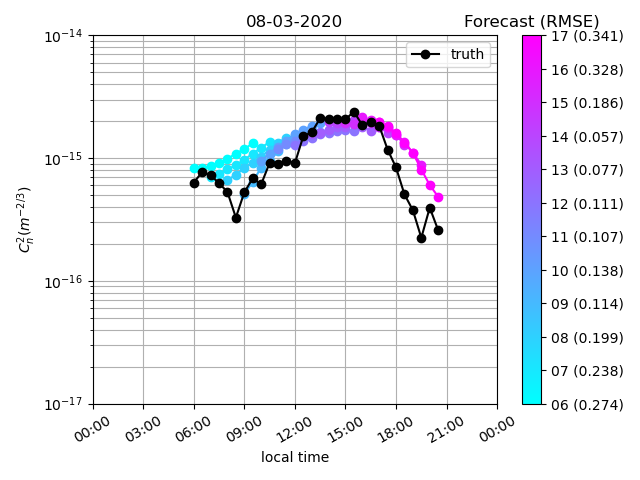
\includegraphics[width=0.49\textwidth]{forecasts_20200803.png}
	}
	\subfloat[August 05\label{fig:test_daily_results0_b}]{
		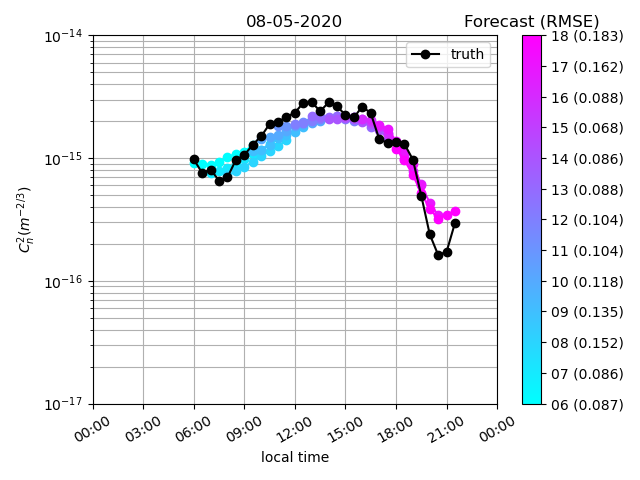
\includegraphics[width=0.49\textwidth]{forecasts_20200805.png}
	}
	\hfill
	\subfloat[August 06\label{fig:test_daily_results0_c}]{
		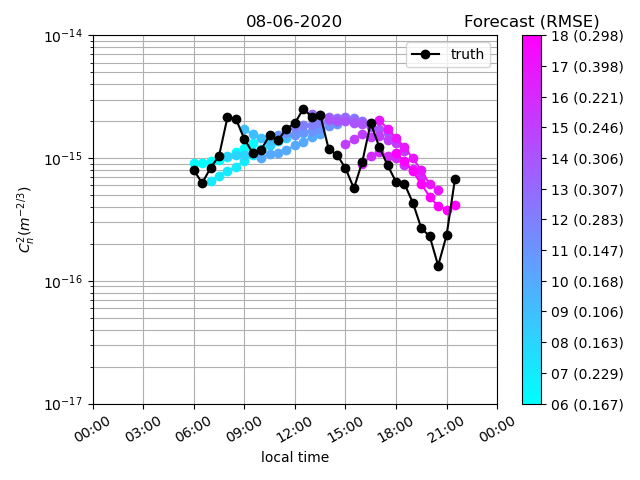
\includegraphics[width=0.49\textwidth]{forecasts_20200806.png}
	}
	\subfloat[August 07\label{fig:test_daily_results0_d}]{
		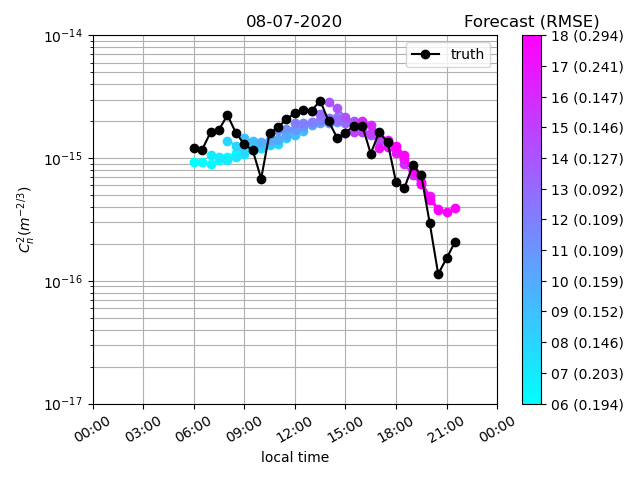
\includegraphics[width=0.49\textwidth]{forecasts_20200807.png}
	}
	\hfill
	\caption{August 3 and 5 - 7 daily $C_{n}^{2}$ forecasts.}
	\label{fig:test_daily_results0}
\end{figure}
For example in Figure \ref{fig:test_daily_results0_a}, the earliest forecast's (furthest left) first timestamp is at 06:00 and is correspondingly labeled in the colorbar as 06. The color of this earliest curve is brightest cyan which is consistent with the label on the colorbar. The error score for this forecast is 0.274. Likewise, the last forecast of the day in Figure \ref{fig:test_daily_results0_a} is at 17:00 and is the brightest magenta curve. The colorbar label is 17 and is the top color in the colorbar. The loss score for this individual forecast is 0.341. Note that in these daily-$C_{n}^{2}$ plots only the forecasts whose first timestamp is at the top of the hour are illustrated. This is done purely for aesthetics to avoid cluttered plots.

The daily-$C_{n}^{2}$ plots in Figure \ref{fig:test_daily_results0} illustrate many unique features. Starting with 08/03 in Figure \ref{fig:test_daily_results0_a}, the morning (cyan) forecasts all forecast a similar trend in $C_{n}^{2}$: a steady rise. Interestingly, the magnitude of the forecasted conditions seems to be different by a scale-factor between the first three forecasts at 06:00 - 08:00. This illustrates the impact of including prior $C_{n}^{2}$ conditions as an input sequence into the model. At the 07:00 and 08:00 forecasts, the model is given information that the most recently measured $C_{n}^{2}$ is trending down in magnitude so the forecasts, while still trending upward, lowers in overall magnitude because the model has learned that its forecasts should start near the most recently measured conditions. This feature is consistently seen throughout all test forecasts. Another interesting feature is the evening forecasts in Figure \ref{fig:test_daily_results0_a}. The 15:00 - 18:00 model forecasts predict $C_{n}^{2}$ to significantly lower in magnitude starting around 18:00 until 20:30. The measured conditions significantly lower, but temporally earlier than predicted. This is a rare case where the model gets the evening neutral event magnitude mostly right but misses the temporal component. Generally, the model on this day forecasts a mostly standard diurnal trend, but the measurements are weather impacted. At 10:00 there is a slight drop in measured turbulence, then from 10:30 - 12:00 the measured conditions are steady around $9 \times 10^{-16} (m^{-2/3})$. A standard diurnal trend occurs from 12:30 to 17:00, and the model accurately forecasts this.

Forecasts on 08/05 in Figure \ref{fig:test_daily_results0_b} are consistent with a standard diurnal trend. Specifically, the forecasts accurately predict the weak morning neutral event indicated by the drop in $C_{n}^{2}$ around 07:00 to 08:00 then a steady rise in strength until 12:00. The forecasts predict slightly lower $C_{n}^{2}$ strength than measured, but the difference is small. The forecasts then accurately predict the drop in $C_{n}^{2}$ strength starting around 15:00. These forecasts are accurate temporally and in strength of neutral event until the deepest part around 21:00. The measured $C_{n}^{2}$ strength continues to drop but the model does not reach this depth. However, the model does accurately forecast the slight rise in $C_{n}^{2}$ at the very end of the day. Every forecast in Figure \ref{fig:test_daily_results0_b} has an error score lower than the error score of 0.1868 from the 10-model ensemble average as applied to the entire test dataset. More specifically, 6 of the 12 forecasts have error scores less than 0.01. These scores indicate that 08/05 is an illustration of great model performance for an entire day.

Model performance on 08/06 in Figure \ref{fig:test_daily_results0_c} is the worst of the seven test days (see Figure \ref{fig:GRU_daily_performance}). The first three forecasts of the day at 06:00 - 08:00 have average to above-average error scores because the forecasts predict a steady rise in $C_{n}^{2}$ strength which generally is measured, but a weather-induced rise in $C_{n}^{2}$ strength at 08:00 is not captured. The 09:00 forecast, which boasts the lowest error score of the day of 0.104, benefits from knowledge of the prior $C_{n}^{2}$ measurements as an input. The forecast starts high, around $2 \times 10^{-15} (m^{-2/3})$, drops down in $C_{n}^{2}$ strength then continues upward in $C_{n}^{2}$ strength with the other forecasts which is accurate with the truth measurements. Forecast performance is poor again starting at 14:00 because another weather-induced turbulence event has occurred, but this time it's a 2-hour drop in $C_{n}^{2}$ strength which the forecasts beforehand do not predict. The 15:00 forecast is the first to see the prior measured $C_{n}^{2}$ conditions which include the weather event and so the model tries to compensate for the suddenly-lower $C_{n}^{2}$ strength by starting lower then rising for a few timestamps to reach the conditions it expects around this time. The 16:00 forecast captures the first timestamp, but misses the very high strength $C_{n}^{2}$ at 15:30, then sharp and consistent drop in $C_{n}^{2}$ as part of the evening neutral event from 15:30 till 20:30. The 17:00 and 18:00 forecasts also miss this long and deep evening neutral event. Overall, 08/06 illustrates where the model struggles: highly-weather impacted conditions.

The fourth test day, 08/07 in Figure \ref{fig:test_daily_results0_d}, illustrates a unique combination of forecasts. In the morning, the model forecasts a slow rise in $C_{n}^{2}$ strength until around 13:00 which is generally consistent with measurements, but does not predict the weather-induced rise in $C_{n}^{2}$ at 08:00 then subsequent drop at 10:00. These two events are very short, only consisting of a single timestamp (30 minutes). After this mini-event, the measured conditions are generally diurnal trend through 19:00. There are a few dips in measured $C_{n}^{2}$ strength but they are high frequency and bounce back to a normal diurnal trend which the model accurately forecasts. The forecasts from 11:00 through 16:00 all have error scores below 0.15, well below the average on the entire test dataset of 0.1868 from the ensemble results. The forecasts at 17:00 and 18:00 have high error scores because the model does not accurately predict the extremely sharp drop in $C_{n}^{2}$ strength from $7 \times 10^{-16} (m^{-2/3})$ at 19:30 to about $1 \times 10^{-16} (m^{-2/3})$ at 20:30, only 1 hour later. These late forecasts accurately predict the slight rise in turbulence at 21:00 and 21:30 after the deepest part of the evening neutral event, but the error scores are high because the model could not reach the depth. The 18:00 forecast is a good example of the model accurately forecasting the temporal nature of turbulence conditions but missing the very low magnitude of the neutral event.

The final three test days, 08/08 - 08/10, are presented in Figures \ref{fig:test_daily_results1_a}, \ref{fig:test_daily_results1_b}, and \ref{fig:test_daily_results1_c}, respectively. On average over the 10-model ensemble study, 08/08 is the second best day of model performance. Throughout the day, the model generally predicts diurnal trend: a slow rise in $C_{n}^{2}$ strength until around 15:00 where conditions steady then start to decrease again. The 09:00 through 13:00 forecasts all yield low error scores with 4 of them below 0.01. The first three forecasts from 06:00 through 08:00 have error scores around the ensemble average due to two factors. The 06:00 forecast first predicts turbulence conditions around $1 \times 10^{-15} (m^{-2/3})$, which is the nighttime filled $C_{n}^{2}$ strength, when the measured conditions are actually low. Then the 06:00 forecast altogether misses the weather-induced sharp rise in turbulence conditions from 07:00 to 08:30. The 07:00 and 08:00 forecasts also miss this high-frequency event. It's not until the 09:00 forecast which has the information about the prior turbulence conditions that the forecasts accurately settle into the diurnal trend.
\begin{figure}[h!]
	\centering
	\subfloat[August 08\label{fig:test_daily_results1_a}]{
		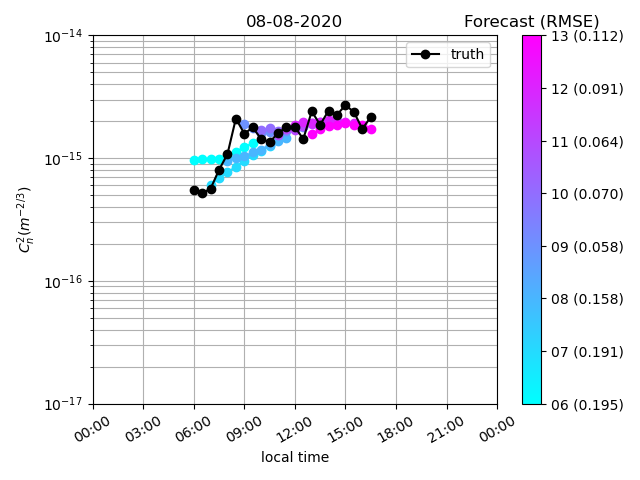
\includegraphics[width=0.49\textwidth]{forecasts_20200808.png}
	}
	\subfloat[August 09\label{fig:test_daily_results1_b}]{
		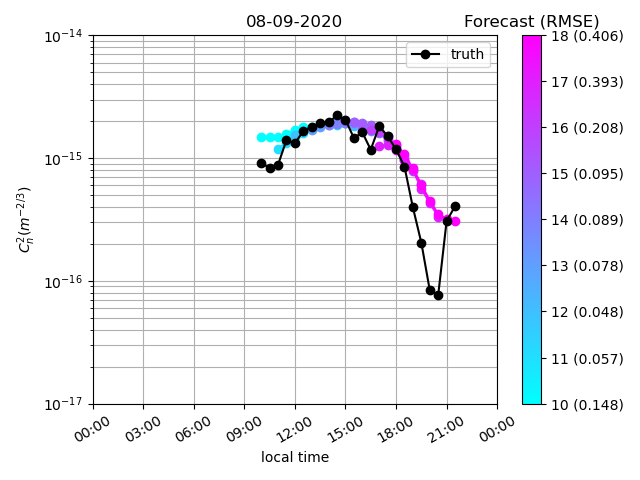
\includegraphics[width=0.49\textwidth]{forecasts_20200809.png}
	}
	\hfill
	\subfloat[August 10\label{fig:test_daily_results1_c}]{
		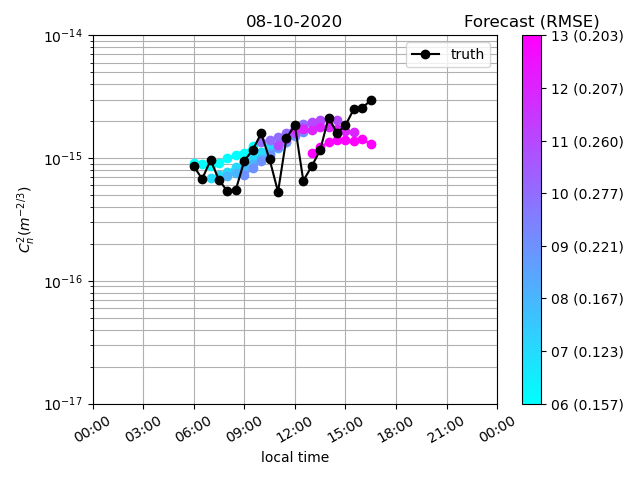
\includegraphics[width=0.49\textwidth]{forecasts_20200810.png}
	}
	\hfill
	\caption{August 8 - 10 daily $C_{n}^{2}$ forecasts.}
	\label{fig:test_daily_results1}
\end{figure}

From the 10-model ensemble study, model performance on 08/09 ranks 4/7 on average and is also one of the most variable from model-to-model (Figure \ref{fig:GRU_daily_performance}). Analysis of the forecast $C_{n}^{2}$ conditions in Figure \ref{fig:test_daily_results1_b} illustrate how an average over the entire day can be misleading. The first forecast at 10:00 has an error score of 0.148 which is below the 10-model overall average, then the 11:00 - 15:00 forecasts each boast error scores less than 0.01.The measured conditions are mostly diurnal and is accurately forecasted by the model. The only deviations are the very slight morning neutral event from 10:00 to 11:00 then a weather-induced slight drop in $C_{n}^{2}$ strength around 16:00. The two forecasts which raise the day's average error score are at 17:00 and 18:00. These forecasts accurately predict the temporal nature of the evening neutral event, but strongly miss the sharp decline and depth of the event. From 18:00 to 20:00, $C_{n}^{2}$ strength drops from just over $1 \times 10^{-15} (m^{-2/3})$ to $8 \times 10^{-17} (m^{-2/3})$, over 1 order-of-magnitude change. In fact, this evening neutral event is just one of only a handful of cases in the entire dataset in which the evening neutral event dips below $1 \times 10^{-16} (m^{-2/3})$ (\textcolor{blue}{count number of individual evening neutral events that reach this threshold? I think there are 7 including test dataset from Figure \ref{fig:forecast_sequence_histogram_a}}). The 17:00 and 18:00 forecasts yield error scores of 0.393 and 0.406, respectively, which are the two highest error scores in the entire test dataset. Beside this uncharacteristically deep neutral event, model performance on 08/09 is well better than average.

The last day of the test dataset, 08/10, is the second worst day of model performance from the 10-model ensemble average in Figure \ref{fig:GRU_daily_performance}. The morning forecasts, which begin at 06:00, generally all predict standard diurnal trends: a slow increase in $C_{n}^{2}$ strength through about 15:00 then a decline. The measured conditions, however, are highly variable both temporally and in $C_{n}^{2}$ strength. Between 06:00 and 15:00 there are five instances of a drop in $C_{n}^{2}$ strength. Likely, at least four of them are weather-induced (possible the 08:00 is morning neutral event). The model forecasts a diurnal trend which follows the trend of the high-strength $C_{n}^{2}$ points over this time period. The 12:00 and 13:00 forecasts predict $C_{n}^{2}$ strength to lower as the afternoon moves into early evening, but the measured conditions actually rise to the highest point in the entire day from 15:30 to 16:30. The 13:00 forecast starts at a lower $C_{n}^{2}$ strength than the surrounding forecasts due to the model having the input sequence information about the very low $C_{n}^{2}$ strength at 12:30. This day again illustrates the the model's inability to accurately forecast high-frequency weather-induced $C_{n}^{2}$ fluctuations. Instead, the model has learned a trend in $C_{n}^{2}$ based on the time of day. The model has also learned to adjust its starting $C_{n}^{2}$ strength based on prior $C_{n}^{2}$ measurements, then settle back into the expected trend. 

\section{Forecast Analysis}
The model forecasts and corresponding truth measurements from Figures \ref{fig:test_daily_results0} and \ref{fig:test_daily_results1} are rearranged by forecast length. Figure \ref{fig:test_scatter_results} presents a scatter plot of measured $C_{n}^{2}$ on the x-axis and forecasted $C_{n}^{2}$ on the y-axis for each time in the 4-hour model forecasts: 0.5 hour, 1 hour, 1.5 hour, and so on through 4 hours. In each scatter plot, the black markers are the truth values plotted as measured $C_{n}^{2}$ vs. measured $C_{n}^{2}$ to yield the linearly arranged markers. The green markers are the model forecast at the scatter plot's designated forecast time plotted as forecasted $C_{n}^{2}$ vs. measured $C_{n}^{2}$.
\begin{figure}[p!]
	\centering
	\subfloat[\label{fig:test_scatter_results_a}]{
		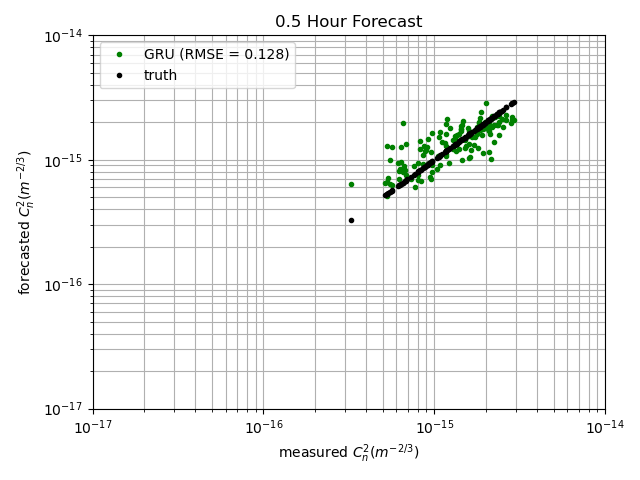
\includegraphics[width=0.40\textwidth]{scatter_0p5hr.png}
	}
	\subfloat[\label{fig:test_scatter_results_b}]{
		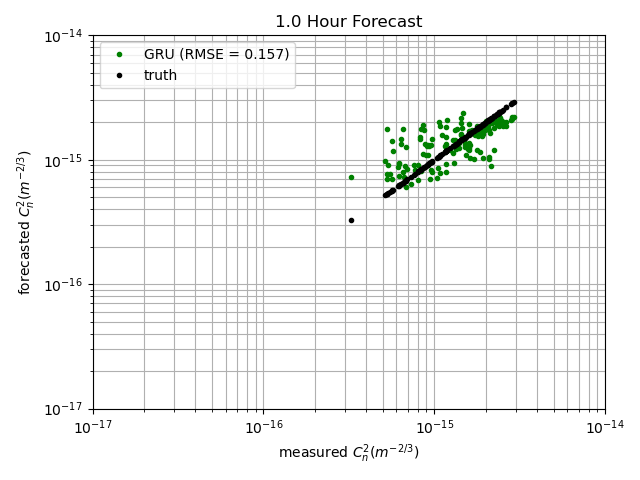
\includegraphics[width=0.40\textwidth]{scatter_1p0hr.png}
	}
	\hfill
	\subfloat[\label{fig:test_scatter_results_c}]{
		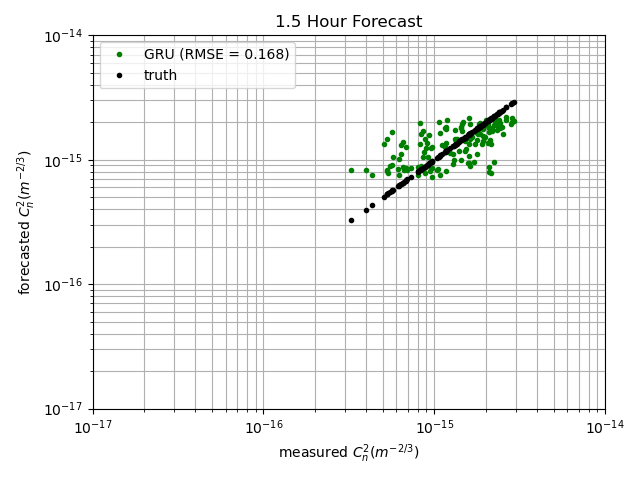
\includegraphics[width=0.40\textwidth]{scatter_1p5hr.png}
	}
	\subfloat[\label{fig:test_scatter_results_d}]{
		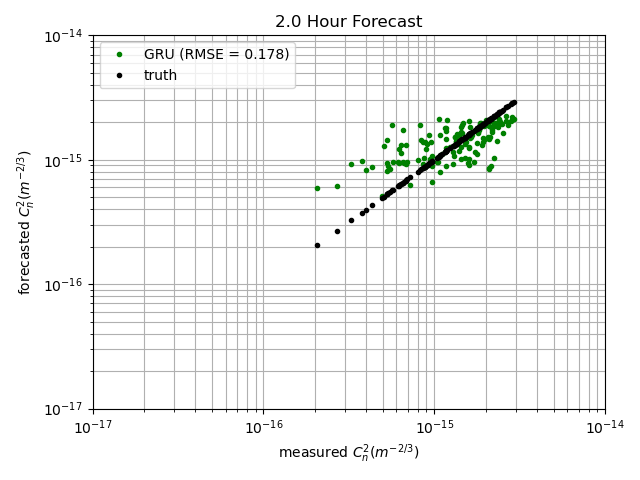
\includegraphics[width=0.40\textwidth]{scatter_2p0hr.png}
	}
	\hfill
	\subfloat[\label{fig:test_scatter_results_e}]{
		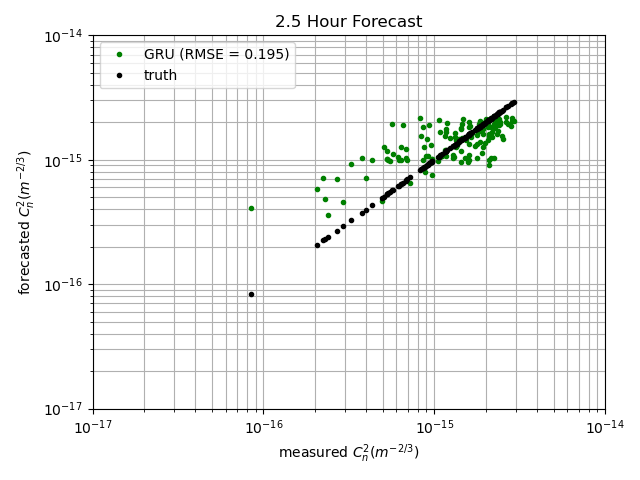
\includegraphics[width=0.40\textwidth]{scatter_2p5hr.png}
	}
	\subfloat[\label{fig:test_scatter_results_f}]{
		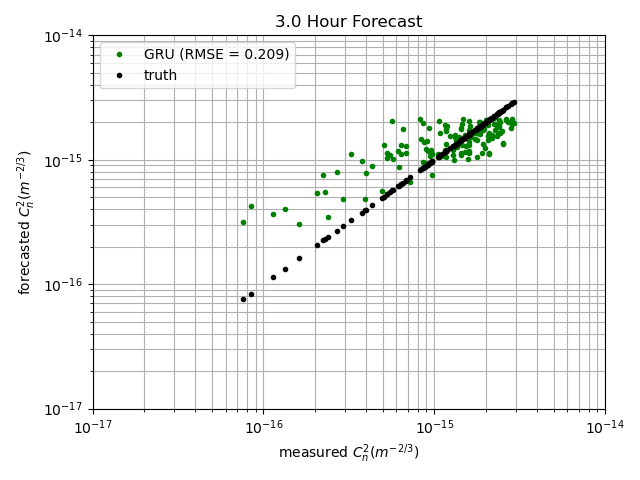
\includegraphics[width=0.40\textwidth]{scatter_3p0hr.png}
	}
	\hfill
	\subfloat[\label{fig:test_scatter_results_g}]{
		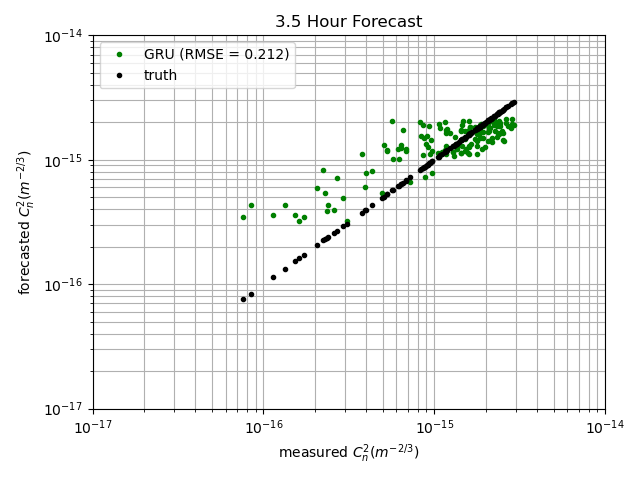
\includegraphics[width=0.40\textwidth]{scatter_3p5hr.png}
	}
	\subfloat[\label{fig:test_scatter_results_h}]{
		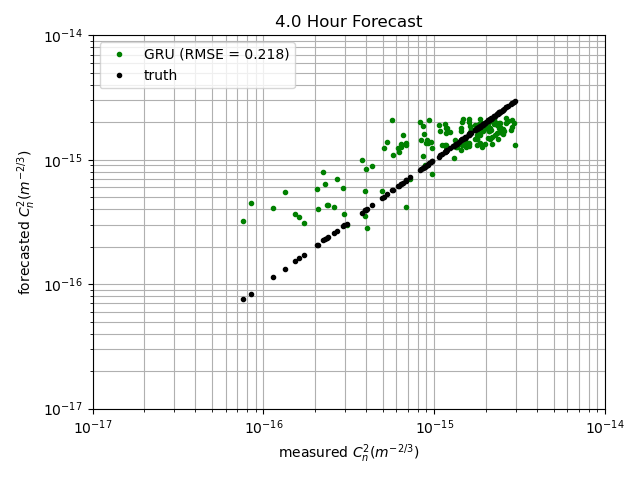
\includegraphics[width=0.40\textwidth]{scatter_4p0hr.png}
	}
	\hfill
	\caption{Scatter plots.}
	\label{fig:test_scatter_results}
\end{figure}
These scatter plots are visually evaluated by how closely the green markers cluster around the black markers. A set that is well clustered around the black points is better than a set that is not well clustered. If the model was perfect, the black markers would directly overlay the green markers. As a quantitative metric of model performance at each forecast hour the average $log_{10}(C_{n}^{2})$ RMSE loss is reported in each legend.

The scatter plot of the first forecast time, 30 minutes, in Figure \ref{fig:test_scatter_results_a} shows a strong clustering of the model forecasts about the measured $C_{n}^{2}$. Excluding one outlier, the range of measured $C_{n}^{2}$ the model is tasked to forecast is only from $5 \times 10^{-16} (m^{-2/3})$ to $3 \times 10^{-15} (m^{-2/3})$, a narrow window. This forecast time also benefits from being closest to the most recently measured $C_{n}^{2}$ and other input sequence variables. Thus, it is expected for this forecast time to do well overall. The RMSE loss score is 0.128, well below the 10-model ensemble average over the whole dataset of 0.1868. The scatter plot of the second time of the model forecasts, 1 hour, in Figure \ref{fig:test_scatter_results_b} shows a slightly worse performance than the 30 minute forecast time. The set of measured points looks very similar to that of 30 minutes, but the clustering of the green model markers about the black truth markers is not as tight. The error score of 0.157 confirms this visual analysis.

The 1.5 and 2 hour forecasts in Figures \ref{fig:test_scatter_results_c} and \ref{fig:test_scatter_results_d} start to clearly show a different set of measured $C_{n}^{2}$ conditions illustrated by the additional black markers toward the middle and lower left corner of the scatter plots. Most of the green model markers have a reasonable cluster around the mid- and high-strength $C_{n}^{2}$ black markers. However, the model struggles to capture measurements below $7 \times 10^{-16} (m^{-2/3})$ as illustrated by the black markers continuing left on the x-axis below this strength, but the green markers staying above $7 \times 10^{-16} (m^{-2/3})$ on the y-axis in Figure \ref{fig:test_scatter_results_c}. In Figure \ref{fig:test_scatter_results_d} is a similar trend, but a couple of model points are beginning to drop into lower strength $C_{n}^{2}$ conditions. The average error scores continue to climb, reaching 0.168 and 0.179 at the 1.5 and 2 hour forecast times, respectively.

The 2.5 and 3 hour forecasts in Figures \ref{fig:test_scatter_results_e} and \ref{fig:test_scatter_results_f} further shown a different set of measurements the model attempts to forecast. Most notable are the increased number of low-strength $C_{n}^{2}$. As forecast time extends further out the number of evening neutral events included in the examined sets also increases. The clustering of the higher-strength $C_{n}^{2}$ conditions continues to slightly deteriorate. The clustering of the green model markers is not as tight about the black truth markers, and more importantly the slope of these green markers is angling more with respect to the slope of the black markers. At low-strength $C_{n}^{2}$ evening neutral events the model is still struggling to forecast $C_{n}^{2}$ that reaches the measured strength. One positive element of these scatter plots is that there are no green markers which are wildly off from it's corresponding black marker. For example, there are no green modeled markers at $2 \times 10^{-15} (m^{-2/3})$ when it's black marker is nearing $1 \times 10^{-16} (m^{-2/3})$. This means the model has generally learned the turbulence conditions well, understanding when to forecast high, medium, and low-strength $C_{n}^{2}$. The error scores for the 2.5 hour and 3 hour forecasts are 0.197 and 0.211, respectively, which follows the trend of increasing error with forecast length.

Finally, the 3.5 and 4 hour forecasts in Figures \ref{fig:test_scatter_results_g} and \ref{fig:test_scatter_results_h} continue to illustrate the trend shown so far: the set of measured $C_{n}^{2}$ to forecast further evolves to include more evening neutral event low-strength conditions. Interestingly, the group of green model markers around the higher-strength $C_{n}^{2}$ is very well clustered with itself, but is at a significant angle with respect to the black truth markers' angle. The model's struggle to capture the deep neutral events is most clearly observed in Figures \ref{fig:test_scatter_results_g} and \ref{fig:test_scatter_results_h}. The model still has learned when to forecast low-strength $C_{n}^{2}$, but cannot reach the required depth. The average loss scores for the 3.5 and 4 hour forecasts are 0.212 and 0.214, respectively.

%The lowest-strength $C_{n}^{2}$ forecasted by the model in the entire test dataset is $3 \times 10^{-16} (m^{-2/3})$ when there are multiple measurements weaker than this level.

Summarizing the scatter plot error scores from Figure \ref{fig:test_scatter_results} is Figure \ref{fig:performance_forecast_length} which plots the loss scores as a function of forecast length. The plot illustrates that as the forecast length increases so does the model performance error. This is an expected result as any forecasting application is expected to decline in performance as forecast time increases.
\begin{figure}[h!]
	\centering
	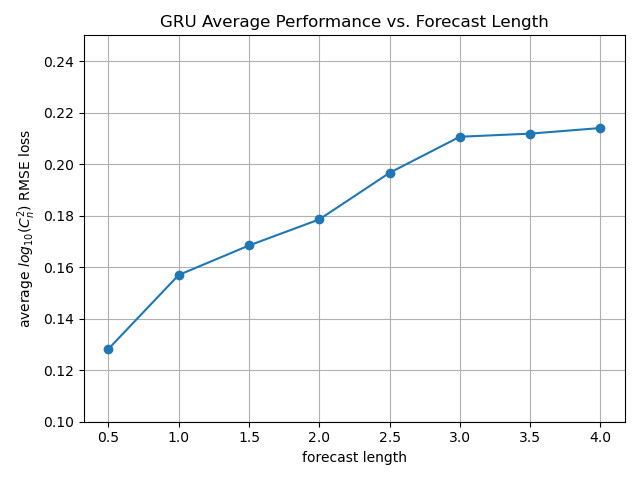
\includegraphics[width=0.65\textwidth]{performance_forecast_length.png}
	\caption{Average performance as a function of forecast length.}
	\label{fig:performance_forecast_length}
\end{figure}

\section{Individual Forecast Analysis}
A final analysis of this model is to understand why it performs well and poorly in specific cases. The section uses the cumulative distribution function (CDF) to statistically illustrate the model's strengths and weaknesses. The CDF is a tool which sorts the given data by magnitude then assigns each sorted data point a percentile from zero (noninclusive) to one (inclusive). The percentile represents the percentage of data points that are less than or equal to the data point's magnitude.

\subsection{2020/08/09 18:00}
A single trend has been abundantly clear throughout the model analysis: the model struggles to capture the deep evening neutral events. In Section \ref{sec:daily_cn2_forecasts} Figure \ref{fig:test_daily_results1_b} the single worst model forecast in terms of RMSE is the 08/09 18:00 forecast. This is the latest forecast of the day (and all days) and the deep neutral event was noted to be one of the deepest of the entire dataset, making it an excellent candidate for further analysis which goes as follows.

First, every forecast and input sequence from the train dataset whose first timestamp matches the forecast in question, 18:00, is gathered. There are a total of 40 train forecasts whose first timestamp matches this criteria. Next, the 40 train forecasts are sorted by measured (truth) $C_{n}^{2}$ magnitude at each timestamp in the 4-hour forecast, so in this case that yields a 40 x 8 \textcolor{blue}{should this be in non-plain text?} array where each column is sorted. The CDF is then computed per timestamp, yielding eight CDFs in this case where percentiles are associated with specific $C_{n}^{2}$ strengths. Finally, the CDFs of $C_{n}^{2}$ values are interpolated to desired percentiles of  20\%, 50\%, and 80\% for each timestamp, yielding a 3 x 8 array of $C_{n}^{2}$ values. 

The next step in this process applies the trained model to the 40 input sequences from the \textbf{train} dataset which results in 40 model forecasts that correspond with the 40 model forecasts just evaluated to CDF 20\%, 50\%, and 80\%. The exact same process just described - sorting the $C_{n}^{2}$ values per timestamp, calculating the CDF, then interpolating to the desired percentiles - is performed on the 40 train dataset model forecasts.

Figure \ref{fig:analysis_08091800} illustrates this analysis. $C_{n}^{2}$ is plotted as a function of local time of day, and the only forecasts considered are those whose first timestamp is at 18:00. The black markers represent the train dataset truth (measured) $C_{n}^{2}$ at each timestamp in the forecast time being evaluated. Thus, at 18:00, 18:30, and so on through 21:30, there are 40 black markers for each time.
\begin{figure}[h!]
	\centering
	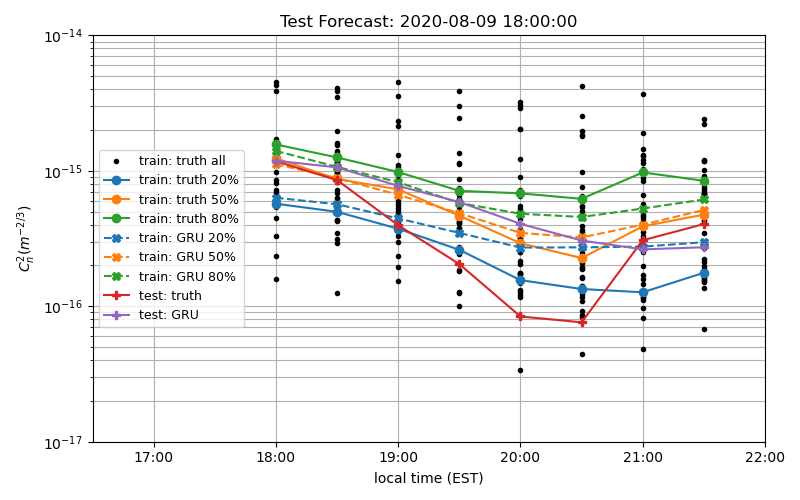
\includegraphics[width=0.85\textwidth]{analysis_202008091800.png}
	\caption{GRU performance analysis of the 08/09 18:00 forecast.}
	\label{fig:analysis_08091800}
\end{figure}

\begin{figure}[h!]
	\centering
	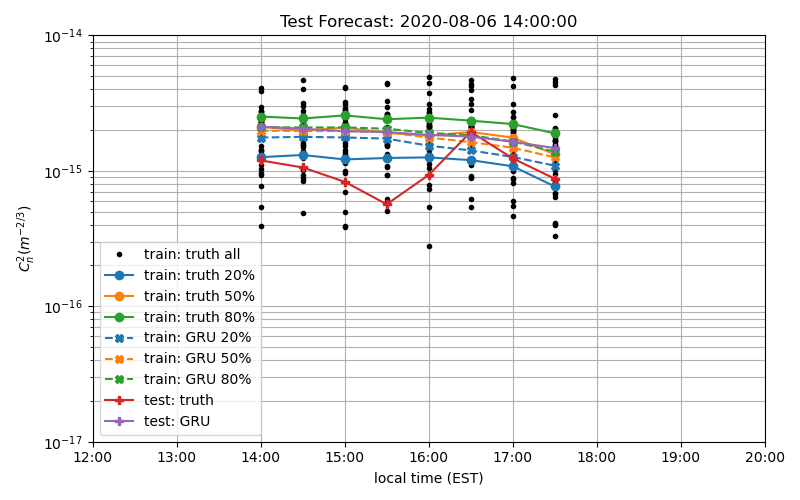
\includegraphics[width=0.65\textwidth]{analysis_202008061400.png}
	\caption{GRU performance analysis of the 08/06 14:00 forecast.}
	\label{fig:analysis_08061400}
\end{figure}

\begin{figure}[h!]
	\centering
	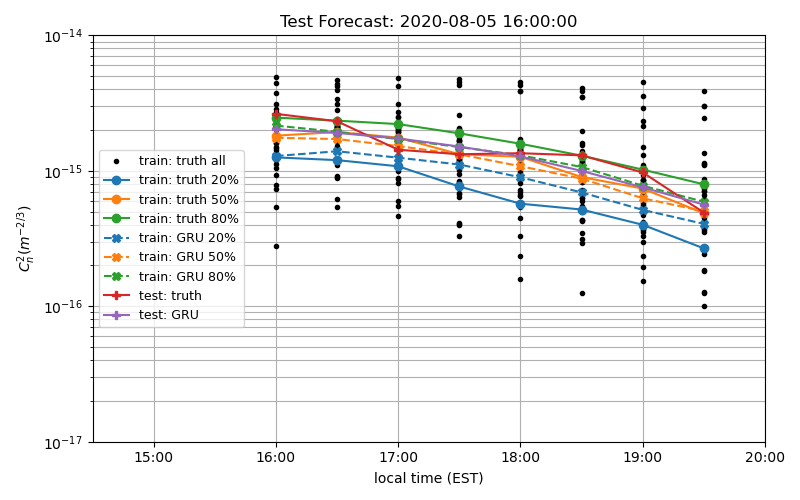
\includegraphics[width=0.65\textwidth]{analysis_202008051600.png}
	\caption{GRU performance analysis of the 08/05 16:00 forecast.}
	\label{fig:analysis_08051600}
\end{figure}